
\section{Methodology}

\subsection{Simulation Environment and Network}

All experiments use one fixed topology: a bidirectional $3\times4$ signalised mesh with 12
signalised junctions, 47 external links and 29 legal simple primary paths
(Fig.~\ref{fig:network}). The upper, central and lower corridors have speed limits of 40,
50 and 60\,km/h and one, one and two lanes, so the three east--west corridors differ in
both free-flow speed and capacity, and three alternative eastbound locations carry a
150\,m speed-restriction segment with a speed ratio of 0.35. Signals run a common 60\,s
cycle: the balanced plan allocates approximately 26\,s each to the competing east--west
and north--south movements, the arterial-priority plan 36\,s and 16\,s, with identical
clearance intervals. Four background streams load the north--south movements that compete
with the primary corridors, and a three-lane source and sink ensure that neither end of
the corridor is the binding constraint. Lane counts are specified design inputs, not
calibrated saturation flows, which limits the external interpretation of absolute values.
Simulation uses SUMO~\cite{lopez2018sumo} with teleporting disabled, so a vehicle that
cannot be inserted waits rather than disappearing from the accounting.
Table~\ref{tab:config} lists the configuration.

\begin{figure}[tb]
\centering
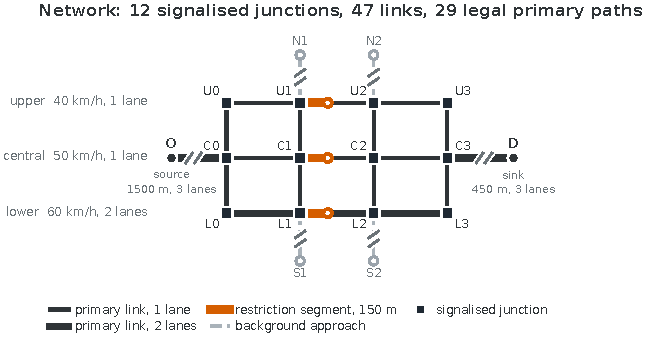
\includegraphics[width=\linewidth]{figures/fig1_network.pdf}
\caption{The fixed network. Line weight encodes lane count, the three alternative
restriction segments are highlighted, and background approaches are dashed with their
stubs shortened at the break marks. Exactly one restriction segment is active in a
restricted context. The 24 contexts built on this network are shown in
Fig.~\ref{fig:regime}b.}
\label{fig:network}
\end{figure}

\begin{table}[htb]
\centering\small
\caption{Simulation configuration. Every item is common to all 432 runs; the factors that
vary between contexts are listed in Section~5.1.}
\label{tab:config}
\begin{tabularx}{\linewidth}{@{}>{\raggedright\arraybackslash}p{0.26\linewidth}R@{}}
\toprule
Item & Setting\\
\midrule
Network & Bidirectional $3\times4$ mesh; 12 signalised junctions; 47 external links; 29
legal simple paths; 400\,m horizontal and 300\,m vertical spacing\\
Corridors & Upper 40\,km/h, 1 lane; central 50\,km/h, 1 lane; lower 60\,km/h, 2 lanes\\
Signal cycle & 60\,s, with two 3\,s yellow and 1\,s all-red clearance intervals\\
Background demand & Four north--south streams, 200\,veh/h each\\
Simulator and fleet & SUMO, 1\,s step, teleporting disabled; homogeneous fleet, HBEFA3
\texttt{PC\_G\_EU4}\\
Restriction segment & 150\,m, speed ratio 0.35, in one of three alternative eastbound
locations\\
Signal plans & balanced 26/26\,s; arterial-priority 36/16\,s\\
Measurement window & 600\,s warm-up; primary requests generated to 2400\,s and followed
to arrival\\
\bottomrule
\end{tabularx}
\end{table}

\subsection{Routing Policy Portfolio}

Let $\mathcal{P}$ be the 29 admissible paths, $L(p)$ the static length of path $p$, and
$\widehat T_t(p)$, $\widehat E_t(p)$ the travel-time and emission estimates available at
decision time $t$. The implemented objectives are
\begin{align}
p_{\mathrm{SP}}&\in\arg\min_{p\in\mathcal{P}} L(p), &
p_{\mathrm{DTT}}&\in\arg\min_{p\in\mathcal{P}} \widehat T_t(p),\\
p_{\mathrm{ECO}}&\in\arg\min_{p\in\mathcal{P}} \widehat E_t(p), &
p_{\mathrm{TECO},\alpha}&\in\arg\min_{\{p\,:\,\widehat T_t(p)\le(1+\alpha)\min_q \widehat T_t(q)\}}
\widehat E_t(p),
\end{align}
with $\alpha\in\{0.05,0.10,0.15\}$. These are finite-candidate implementations of
established objectives~\cite{dijkstra1959note,boriboonsomsin2012ecorouting,zeng2017svm,%
huang2018ecorouting}, not new routing algorithms, and the three TECO settings are
parameter values of one family rather than three principles.

\begin{table}[htb]
\centering\small
\caption{Routing policies, their objectives and their role in the analysis.}
\label{tab:policies}
\begin{tabularx}{\linewidth}{@{}>{\raggedright\arraybackslash}p{0.12\linewidth}
>{\raggedright\arraybackslash}p{0.30\linewidth}R@{}}
\toprule
Policy & Objective & Role\\
\midrule
SP & Minimise static path length & Decision portfolio\\
DTT & Minimise estimated travel time on the latest observed interval & Decision
portfolio\\
TECO10 & Minimise estimated \CO\ subject to a 10\,\% travel-time budget & Decision
portfolio\\
TECO05, TECO15 & The same objective, 5\,\% and 15\,\% budgets & Allowance sensitivity;
measured, outside the portfolio\\
ECO & Minimise estimated \CO, no time budget & Negative control; removed by a
route-ordering gate applied before any decision analysis\\
\bottomrule
\end{tabularx}
\end{table}

Every policy uses the same network, demand manifest, signal plan, fleet and admissible
catalogue, so the only difference between two runs of one context is the objective used to
pick a path. Estimates come from completed 60\,s observation intervals, so a request at
time $t$ can see neither the future nor the requesting vehicle's own realised trip; each
vehicle receives one route at departure and does not re-route; compliance is complete. The
exclusion of ECO is a pre-decision screening step reported in Section~\ref{sec:robust}:
its emission forecasts were accurate in aggregate yet ranked routes badly, so it was
removed before the portfolio was analysed and retained as an audited negative control. The
decision portfolio is therefore $\mathcal{A}=\{\text{SP},\text{DTT},\text{TECO10}\}$.

\subsection{Decision Criteria}

Two criteria are primary: mean journey time of the measured cohort, from requested
departure to arrival, and mean tailpipe \CO\ per vehicle of the same cohort. Journey time
therefore includes insertion delay incurred when the network cannot immediately accept a
vehicle, whereas in-network \CO\ excludes pre-insertion idling because a vehicle that has
not entered emits nothing in the model. This asymmetry is a measurement boundary rather
than an error, and its effect on every decision is measured in Section~\ref{sec:robust}.
Fuel is excluded: in this homogeneous fleet it is proportional to \CO\ to within numerical
precision.

Network stopped vehicle-time is a congestion diagnostic rather than a primary criterion,
because it is accumulated over \emph{all} vehicles including background traffic and is
therefore a system-level quantity rather than a service level experienced by the measured
cohort; promoting it after the fact would silently change what ``preferred policy'' means.
The primary two-criterion rule is used unchanged for every regret and headroom quantity in
this paper, and stopped vehicle-time enters a separate, explicitly labelled multi-criteria
analysis in Section~\ref{sec:multicriteria}. Route distance and the 95th percentile of
journey time are likewise diagnostics. Equal weights are used for the two primary
criteria, and the references $r_k$ are their grand means over all contexts and portfolio
policies: 542.844\,s and 1263.515\,g.

\subsection{Decision Cost and Regret}

Criterion means are computed within each run and then averaged over the three paired
replications of a context before Eq.~\eqref{eq:cost} is applied, so a context contributes
one cost per policy. The seeds are paired across policies --- seed $j$ drives the same
exogenous demand realisation whichever policy is active --- so a difference between two
policies in one context is a paired difference. Two conventions affect the reported
values: the references $r_k$ are computed once on the full benchmark for scoring, while in
every held-out protocol the model and its internal scales are refitted on training
contexts only (Section~\ref{sec:robust} reports what happens when the scoring scales are
restricted too); and the best fixed policy is identified inside each fold, so the fixed
baseline is itself a fitted quantity rather than an oracle.

\subsection{Context-Aware Policy Selection}

The selector predicts the criterion outcomes of every portfolio policy from the context
and then applies Eq.~\eqref{eq:cost} to the predicted outcomes. Its inputs are the
scheduled demand, the planned restriction configuration and the signal plan; no realised
outcome of any kind enters the feature vector, and all features are known before any
vehicle departs.

Rather than reporting one model, we evaluate a ladder of rules of increasing capacity
under the same held-out protocol, listed in Table~\ref{tab:ladder}: the single best fixed
policy identified on each fold's training contexts (R0), which adaptation must beat; a
mechanistic demand threshold choosing SP below a fitted value and DTT above it (R1) and
the same rule with one threshold per signal plan (R2); multi-output regression trees of
depth 1 (R3) and of depth 3 with minimum leaf size 2, the pre-registered
setting~\cite{breiman2017cart} (R4); and the hindsight best as an upper bound (R5). R1 and
R2 are explicit rules whose only free parameters are demand thresholds fitted by
minimising training regret, so including them attributes any advantage of R4 to model
capacity rather than to the regime structure itself; the comparison is reported whichever
way it falls.

\subsection{Validation and Robustness}
\label{sec:validation}

The primary held-out protocol is leave-one-context-out: for each held-out context the
model, its reference scales and the identity of the best fixed policy are refitted from
the remaining 23 contexts, and all three replications of the held-out context stay
together. Three further protocols probe different failure modes --- leave-one-demand-out,
which removes an entire demand level and therefore tests behaviour outside the fitted
support; seed-block evaluation, fitting on two seeds and scoring on the third; and a
training-only scaling variant, which removes the last dependence of the score on held-out
data. The sensitivity checks and the two negative controls are listed in Section~5.4 and
reported in Table~\ref{tab:robust}.
